%% Journal of Open Research Software Latex template -- Created By Stephen Bonner and John Brennan, Durham Universtiy, UK.

\documentclass{jors}
\usepackage{amsmath,amssymb}
\usepackage[backend=biber,url=true,doi=true,sorting=none]{biblatex}
\usepackage{hyperref}
\usepackage{tikz}
\usepackage{graphicx}
\usepackage{listings}
\usepackage{color}

\bibliography{vampy}
\lstset{language=Python}
\renewcommand{\lstlistingname}{Algorithm}

%% Set the header information
\pagestyle{fancy}
\definecolor{mygray}{gray}{0.6}
\renewcommand\headrule{}
\rhead{\footnotesize 3}
\rhead{\textcolor{gray}{UP JORS software Latex paper template version 0.1}}

\begin{document}

{\bf Software paper for submission to the Journal of Open Research Software} \\

To complete this template, please replace the blue text with your own. The paper has three main sections: (1) Overview; (2) Availability; (3) Reuse potential. \\

Please submit the completed paper to: editor.jors@ubiquitypress.com

\rule{\textwidth}{1pt}

\section*{(1) Overview}

\vspace{0.5cm}

\section*{Title}

VaMpy: A Python Package to Solve 1D Blood Flow Problems

\section*{Paper Authors}

1. Diem, Alexandra K.; \\
2. Bressloff, Neil W.

\section*{Paper Author Roles and Affiliations}
1. Institute for Complex Systems Simulation \& Computational Engineering and Design, Faculty of Engineering and the Environment, University of Southampton, UK \\
2. Computational Engineering and Design, Faculty of Engineering and the Environment, University of Southampton, UK

\section*{Abstract}
Finite-differences methods such as the Lax-Wendroff method (LW) are commonly used to solve 1D models of blood flow. These models solve for blood flow and lumen area and are useful in disease research, such as hypertension and atherosclerosis, where flow and pressure are good indicators for the presence of disease. Despite the popularity of the LW method to solve the blood flow equations, no implementation a LW solver for these equations has been published and made publicly available. This leads to the re-implementation of the same methods within different research groups and makes verification of results more difficult. The Vascular Modelling in Python (VaMpy) toolkit is a Python package that aims to fill this gap. It implements Richtmyer's two-step Lax-Wendroff scheme to solve 1D model equations of blood flow in arterial trees and aims at facilitating the solution of blood flow problems for various medical applications.

\section*{Keywords}
Python; blood flow; arterial tree; hemodynamics; finite differences; partial differential equations

\section*{Introduction}

One-dimensional (1D) modelling of the cardiovascular system is useful in predicting and understanding the dynamics of blood pressure propagation \cite{Olufsen2000,Sherwin2003a,Alastruey2007,Kolachalama2007,Cousins2014,Diem2016a}. Here, arteries are regarded as 1D axisymmetric tubes that are described by flux $q$ inside the lumen and cross-sectional area $A$ of the vessel lumen along the vessel length. One popular finite-differences method to numerically solve the equations governing blood flow through arteries is Richtmyer's two-step Lax-Wendroff method \cite{LeVeque1992,Richtmyer1963}, which has been used by a number of groups \cite{Olufsen2000,Kolachalama2007,Diem2016a,Smith2002,Azer2007,Itu2011}. Alternative methods of solving the blood flow equations include for example variations of the Galerkin finite-element method, which instead solve the blood flow equations for flow velocity $u$ and cross-sectional area $A$ \cite{Sherwin2003a,Mynard2008}.

The computational implementation of the Lax-Wendroff method is straightforward and previously mentioned references have produced results that are validated against experimental results, justifying the popularity of the method. However, no openly available implementation of the Lax-Wendroff method could be found, which results in the same work being carried out numerous times. Whilst one open-source Python package implementing a haemodynamic model exists, pyNS focusses on the implementation of a 0D pulse wave propagation model, representing arteries as electrical circuits \cite{Manini2015}, and therefore its scope and application are different from VaMpy. Solutions computed using VaMpy are exported to the commonly used CSV file format, thereby allowing for the integration of data with most other software. For example, solutions calculated using VaMpy could be used as a boundary condition for higher order models of larger arteries further upstream.

\begin{figure}
  \center
  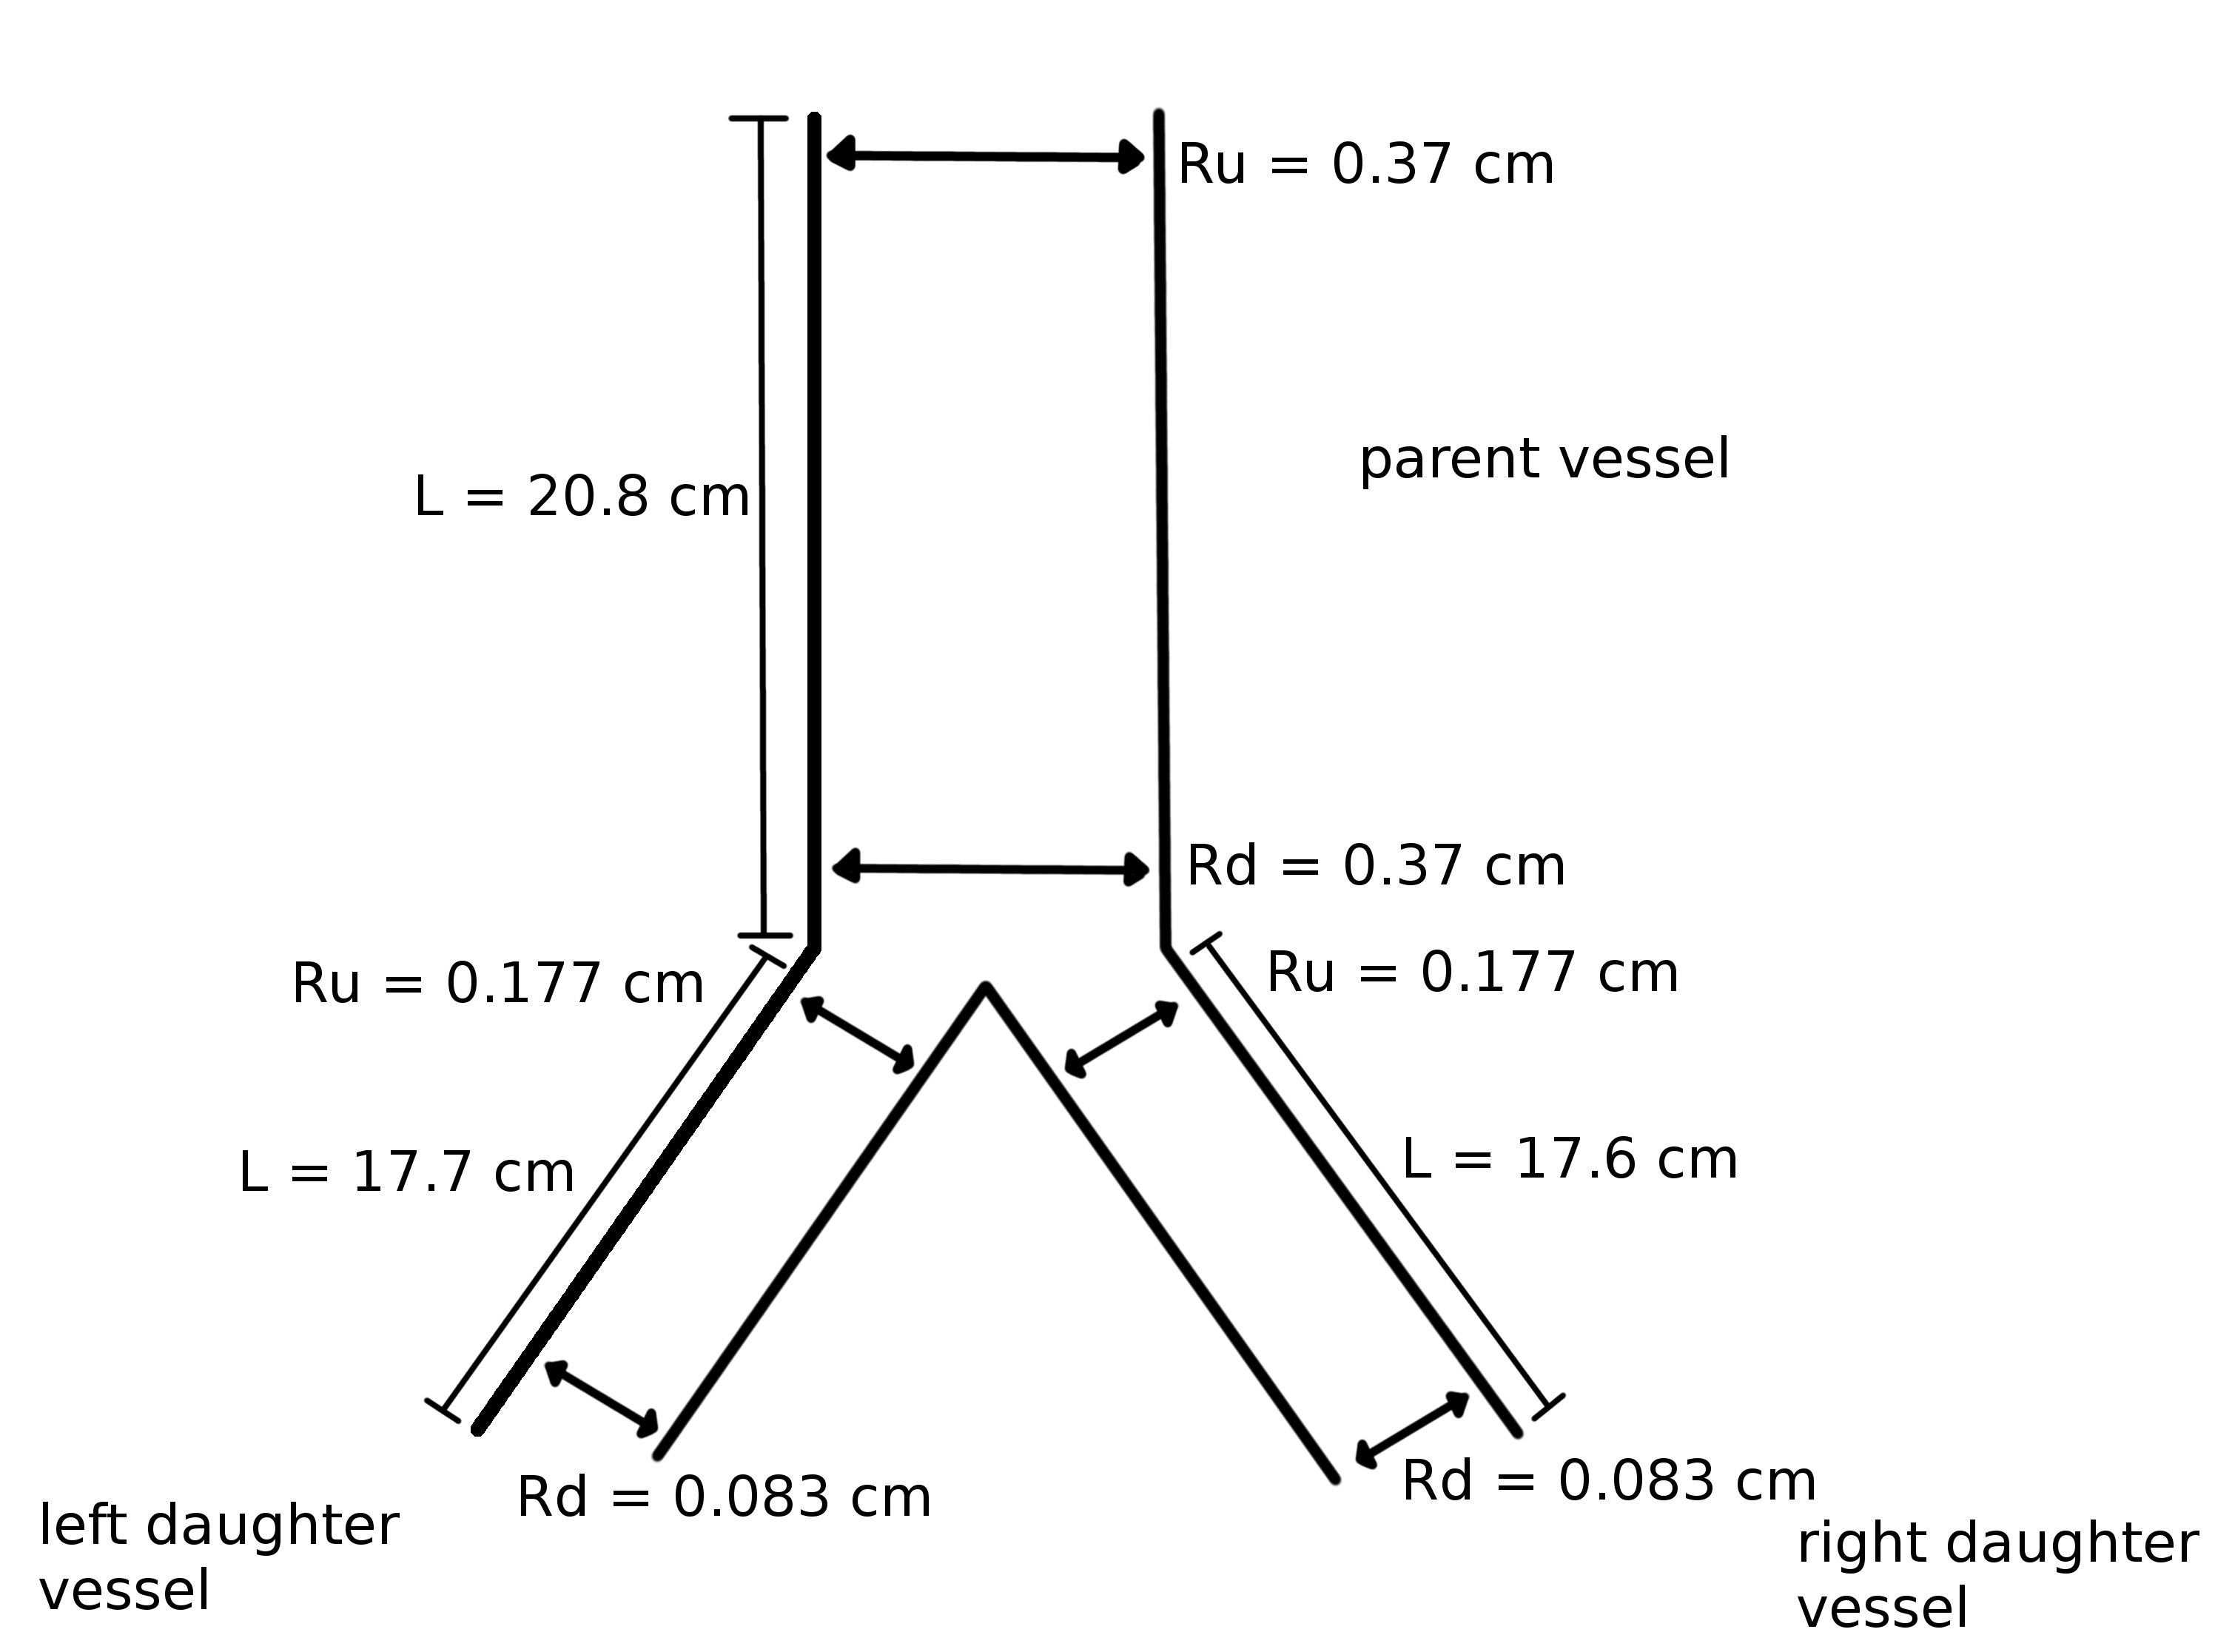
\includegraphics[width=\linewidth]{figures/geometry.png}
  \caption{Example geometry of a bifurcation implemented in VaMpy. The example represents the common carotid artery (parent vessel) and its two daughter vessels, which are used for validation purposes of the software. Artery segments have an upstream and downstream radius, where the downstream radius has to be equal to or smaller than the upstream radius. The radius of the vessel then is $r_0(z) = R_u \cdot \exp ( \log ( R_d/R_u ) \; z/L )$. \label{fig:geometry}}
\end{figure}

Arteries are considered to be elastic axisymmetrical tubes of initial radius $r_0(z)$ in a cylindrical coordinate system. The radius at rest is allowed to taper exponentially for an arterial segment if different values are given for the upstream radius $R_u$ and downstream radius $R_d$. An example geometry for the bifurcation of the common carotid artery, which is used to validate the solution calculated by VaMpy is shown in Figure~\ref{fig:geometry} Then the vessel radius for an arterial segment of length $L$ is
\begin{equation}
r_0(z) = R_u \cdot \exp \left( \log \left( \frac{R_d}{R_u} \right) \frac{z}{L} \right).
\end{equation}
Blood flow through arteries is governed by the Navier-Stokes equations for conservation of mass (continuity equation) and momentum in a 1D cylindrical coordinate system
\begin{gather}
\frac{\partial u_z(r,z,t)}{\partial z} + \frac{1}{r} \frac{\partial \left( ru_r(r,z,t) \right)}{\partial t} = 0\\
\begin{split}
\frac{\partial u_z(r,z,t)}{\partial t} + u_z(r,z,t) \frac{\partial u_z(r,z,t)}{\partial z} + u_r(r,z,t) \frac{\partial u_z(r,z,t)}{\partial r} + \frac{1}{\rho} \frac{\partial p(z,t)}{\partial z} =&\\
\frac{\nu}{r} \frac{\partial}{\partial r} \left( r \frac{\partial u_z(r,z,t)}{\partial r} \right) &,
\end{split}
\end{gather}
where $\boldsymbol{u} = (u_z(r,z,t), u_r(r,z,t))$ denotes blood flow veloctiy, $p(z,t)$ denotes blood pressure, which is assumed to be uniform across $r$ and the parameters $\rho$ and $\nu$ denote blood density and viscosity, respectively. By integration of the governing equations over cross-sectional area $A(z,t) = \pi R(z,t)^2$ the 1D conservation law
\begin{equation}\label{eq:conservation}
\frac{\partial \boldsymbol{U}}{\partial t} + \frac{\partial \boldsymbol{F}}{\partial z} = \boldsymbol{S}
\end{equation}
with  
\begin{gather*}
  \boldsymbol{U} = \begin{pmatrix} A(z,t) \\ q(z,t) \end{pmatrix}, \quad \boldsymbol{F} = \begin{pmatrix} q(z,t)\\ \dfrac{q(z,t)^2}{A(z,t)} + f(r_0) \sqrt{A_0(z) A(z,t)} \end{pmatrix}, \quad \boldsymbol{S} = \begin{pmatrix} 0\\ S_1 \end{pmatrix}\\
  \begin{split}
    S_1 = -&\frac{2 \pi R(z,t)}{\delta_b \mathrm{Re}} \frac{q(z,t)}{A(z,t)} +\\
    &\left( 2 \sqrt{A(z,t)} \left( \sqrt{\pi} f(r_0) + \sqrt{A_0(z)} \frac{df(r_0)}{dr_0 } \right) - A(z,t) \frac{df(r_0)}{dr_0} \right) \frac{dr_0(z)}{dz}
  \end{split}
\end{gather*}
can be derived. Details on the derivation of \eqref{eq:conservation} can be found elsewhere \cite{Olufsen2000,Diem2016a}. Here, the unknowns are the vessel cross-sectional area $A(z,t)$ and flux $q(z,t)$. Elasticity of the vessel is described by the quantity $f(r_0)$ with relaxed vessel radius $r_0(z)$, $A_0(z)$ is the relaxed cross-sectional vessel area, $R(z,t)$ the vessel radius, $\delta_b$ is the boundary layer thickness and $\mathrm{Re}$ is the Reynold's number.

\begin{figure}
\center
  \begin{tikzpicture}[node distance=2.5cm,auto,>=latex]
    % coordinate axes
    \node[label=left:{\scriptsize$t$}] (a) {};
    \node[label=left:{\scriptsize$n$}] (b) [below of=a, node distance=3cm, coordinate] {};
    \node (c) [right of=b, node distance=10.0cm] {\scriptsize$z$};
    \path[->] (b) edge node {} (a);
    \path[->] (b) edge node {} (c);
    % axes labels
    \node[label=left:{\scriptsize$n+1/2$}] [below of=a, node distance=2.0cm, coordinate] {};
    \node[label=left:{\scriptsize$n+1$}] [below of=a, node distance=1.0cm, coordinate] {};
    \node (d) [below of=b, node distance=0.7cm, coordinate] {};
    \node[label={\scriptsize$m-2$}, right of=d, node distance=1.0cm, coordinate] {};
    \node[label={\scriptsize$m-1$}, right of=d, node distance=3.0cm, coordinate] {};
    \node[label={\scriptsize$m-\frac{1}{2}$}, right of=d, node distance=4.0cm, yshift=-0.08cm, coordinate] {};
    \node[label={\scriptsize$m$}, right of=d, node distance=5.0cm, coordinate] {};
    \node[label={\scriptsize$m+\frac{1}{2}$}, right of=d, node distance=6.0cm, yshift=-0.08cm, coordinate] {};
    \node[label={\scriptsize$m+1$}, right of=d, node distance=7.0cm, coordinate] {};
    \node[label={\scriptsize$m+2$}, right of=d, node distance=9.0cm, coordinate] {};
    % black at known positions
    \draw[fill=black] (1cm,-3cm) circle (0.1cm);
    \draw[fill=black] (3cm,-3cm) circle (0.1cm); 
    \draw[fill=black] (5cm,-3cm) circle (0.1cm);   
    \draw[fill=black] (7cm,-3cm) circle (0.1cm);  
    \draw[fill=black] (9cm,-3cm) circle (0.1cm);
    % grey circles at half positions
    \draw[fill=gray] (4cm,-2cm) circle (0.1cm);
    \draw[fill=gray] (6cm,-2cm) circle (0.1cm);
    % white circle at unknown position
    \draw (5cm,-1cm) circle (0.1cm);
    % draw lines to indicate where circle is calculated from 
    \draw (3cm,-3cm) -- (4cm,-2cm);
    \draw (5cm,-3cm) -- (4cm,-2cm);
    \draw (5cm,-3cm) -- (6cm,-2cm);
    \draw (7cm,-3cm) -- (6cm,-2cm);
    \draw (4cm,-2cm) -- (5cm,-1cm);
    \draw (5cm,-3cm) -- (5cm,-1cm);
    \draw (6cm,-2cm) -- (5cm,-1cm);
  \end{tikzpicture}
  \caption{Illustration of the LW method. The solution is fully known at time step $n$ (black circles) and we are looking for the solution at grid point $m$ at time step $n+1$ (white circle). To determine the unknown solution, two intermediate solutions at half grid points $m \pm 1/2$ and at half time step $n+1/2$ are determined from grid points $m-1$, $m$ and $m+1$ at current time step $n$. The intermediate solutions are then used in conjunction with the known solution at grid point $m$ and current time step $n$ to calculate the unknown solution at grid point $m$ and next time step $n+1$ \cite{Kolachalama2007}. \label{fig:laxwendroff}}
\end{figure}

Although these equations have been commonly used by various groups \cite{Olufsen2000,Kolachalama2007,Cousins2014,Devault2008}, no publicly accessible implementation of the solution to \eqref{eq:conservation} could be found, meaning that each publication from a separate group resulted in the reimplementation of the same or very similar methods and equations. Therefore, the Vascular Modelling in Python toolkit (VaMpy) was developed and published on GitHub\footnote{\url{https://github.com/akdiem/vampy}} with the documentation available on GitHub Pages\footnote{\url{http://akdiem.github.io/vampy/}}. Support for the use of VaMpy is mainly available via the Issue Tracker feature on GitHub, but also via contacting the authors.

\section*{Implementation and architecture}

The VaMpy implementation and architecture are described in this section. VaMpy is object-oriented to allow for an intuitive understanding of its design and to facilitate the addition of new features. The base of the package is the class ArteryNetwork, which defines the arterial tree. The class contains methods that are applied on the entire network of arteries as well as boundary conditions. Each artery within the tree is defined as an object of the class Artery, which contains its own solver instance. The solver itself is implemented in the independent class LaxWendroff that implements the Lax-Wendroff method as described below. This approach allows for the integration of other solvers within the software.

The code was developed in Python 2.7 and implements Richtmyer's two-step version of the Lax-Wendroff method \cite{LeVeque1992,Richtmyer1963}, which is second-order accurate in time and space. For a point in time, $n$, the solution at the next time step $n+1$ at grid location $m$ is given by
\begin{equation}\label{eq:lw_full}
  \boldsymbol{U}_m^{n+1} = \boldsymbol{U}_m^n - \frac{\Delta t}{\Delta z} \left( \boldsymbol{F}_{m+1/2}^{n+1/2} - \boldsymbol{F}_{m-1/2}^{n+1/2} \right) + \frac{\Delta t}{2} \left( \boldsymbol{S}_{m+1/2}^{n+1/2} + \boldsymbol{S}_{m-1/2}^{n+1/2} \right),
\end{equation}
where $\boldsymbol{U}_m^n = \boldsymbol{U}(m \Delta z, n \Delta t)$ is the solution at position $m \Delta z$ and time $n \Delta t$. The half time step values for $\boldsymbol{F}$ and $\boldsymbol{S}$ are determined by
\begin{equation}\label{eq:lw_half}
  \boldsymbol{U}_j^{n+1/2} = \frac{\boldsymbol{U}_{j+1/2}^n + \boldsymbol{U}_{j-1/2}^n}{2} + \frac{\Delta t}{2} \left( - \frac{\boldsymbol{F}_{j+1/2}^n - \boldsymbol{F}_{j-1/2}^n}{\Delta z} + \frac{\boldsymbol{S}_{j+1/2}^n + \boldsymbol{S}_{j-1/2}^n}{2} \right)
\end{equation}
for $j = m \pm 1/2$. An illustration of the computational procedure to determine $\boldsymbol{U}_m^{n+1}$ is shown in Figure~\ref{fig:laxwendroff}. It illustrates that both initial conditions at $n = 0$ for all $m$ and left and right boundary conditions are required to determine $\boldsymbol{U}$.

Boundary conditions are applied at both ends of the vessel and are either an inlet, outlet or bifurcation condition. The inlet boundary condition is used at the inlet of the parent vessel only \cite{Olufsen2000}. It requires flux values $q(0,t)$ to be prescribed. The inlet area is then calculated according to \eqref{eq:lw_full}
\begin{equation}
A_0^{n+1} = A_0^n - \frac{\Delta t}{\Delta z} \left( q_{1/2}^{n+1/2} - q_{-1/2}^{n+1/2} \right).
\end{equation}
This requires the evaluation of the term $q_{-1/2}^{n+1/2}$, which is estimated from
\begin{equation}
q_{0}^{n+1/2} = \frac{1}{2} \left( q_{-1/2}^{n+1/2} + q_{1/2}^{n+1/2} \right),
\end{equation}
where $q_{0}^{n+1/2}$ is evaluated from the function prescribing flux values at the inlet and $q_{1/2}^{n+1/2}$ is evaluated from \eqref{eq:lw_half}, see also \cite{Olufsen2000,Kolachalama2007}. 

\begin{lstlisting}[frame=single,mathescape,caption={Iterative scheme to determine $\boldsymbol{U}_M^{n+1}$ using a 3WK boundary condition \cite{Kolachalama2007}. An initial guess is made for $p_M^{n+1}$, from which $q_M^{n+1} is calculated using \eqref{eq:3wk}$ and $A_M^{n+1}$ is calculated using the discretized mass conservation equation \eqref{eq:disc_mass}. Using $A_M^{n+1}$ the next iteration of $p_M^{n+1}$ is found via the state equation \eqref{eq:state}. The algorithm stops after $k_\text{max}$ iterations or when the difference between pressure estimates is less than the small threshold value $\epsilon$.}, label=alg:outlet]
$p_M^{n+1} = p_M^n$ # initial guess for $p_m^{n+1}$
$k = 0$
for $k \leq k_\text{max}$:
    $p_\text{old} = p_M^n$
    $q_M^{n+1} = q_M^n + \frac{p_M^{n+1} - p_M^n}{R_1} + \frac{\Delta t p_M^n}{R_1 R_2 C_T} - \frac{\Delta t q_M^n (R_1 + R_2)}{R_1 R_2 C_T}$
    $A_M^{n+1} = A_0^n - \frac{\Delta t}{\Delta z} ( q_M^{n+1} - q_{M-1}^{n+1} )$
    $p_M^{n+1} = f_M^{n+1} \left( 1 - \sqrt{\frac{(A_0)_M}{A_M^{n+1}}} \right)$
    if $| p_\text{old} - p_M^{n+1} | \leq \epsilon$:
        break
    $k = k + 1$
\end{lstlisting}

The outlet boundary condition is a 3WK and its implementation follows \cite{Kolachalama2007}. The 3WK equation is
\begin{equation}\label{eq:3wk}
  \frac{\partial p(z,t)}{\partial t} = R_1 \frac{\partial q(z,t)}{\partial t} - \frac{p(z,t)}{R_2 C_T} + \frac{q(z,t) (R_1 + R_2)}{R_2 C_T},
\end{equation}
where $R_1$, $R_2$ and $C_T$ are resistance and compliance parameters. Discretization of \eqref{eq:3wk} leads to
\begin{equation}
\frac{p_M^{n+1} - p_M^n}{\Delta t} = R_1 \frac{q_M^{n+1} - q_M^n}{\Delta t} - \frac{p_M^n}{R_2 C_T} + \frac{q_M^n (R_1 + R_2)}{R_2 C_T},
\end{equation}
where $M$ is the spatial position of the outlet. The 3WK boundary condition requires the evaluation of pressure in the vessel, which is related to area via the discretized State Equation \cite{Olufsen2000}
\begin{equation}\label{eq:state}
  p_M^{n+1} = f_M^{n+1} \left( 1 - \sqrt{\frac{(A_0)_M}{A_M^{n+1}}} \right).
\end{equation}
The outlet boundary condition is solved using an iterative scheme with an initial guess for $p_M^{n+1}$ (see Algorithm~\ref{alg:outlet}). This requires a discretized version of the mass conservation equation to obtain an estimate for $A_M^{n+1}$
\begin{equation}\label{eq:disc_mass}
A_M^{n+1} = A_0^n - \frac{\Delta t}{\Delta z} \left( q_M^{n+1} - q_{M-1}^{n+1} \right).
\end{equation}

Finally, a bifurcation boundary condition applies between any vessel that is not a terminal vessel and its two daughter vessels \cite{Olufsen2000,Kolachalama2007}. Relations between parent and daughter vessels lead to a system of eighteen equations for eighteen unknowns, which are solved using Newton's method according to
\begin{equation}\label{eq:newton}
\boldsymbol{x}_{k+1} = \boldsymbol{x}_k - (\boldsymbol{J}(\boldsymbol{x}_k))^{-1} \boldsymbol{f_J}(\boldsymbol{x}_k) \qquad \text{for } k = 0, 1, 2, \ldots
\end{equation}
where $k$ indicates the current iteration, $\boldsymbol = (x_1, x_2, \ldots, x_{18})$, $\boldsymbol{J}(\boldsymbol{x}_k))$ is the Jacobian of the system of equations and $\boldsymbol{f_J}(\boldsymbol{x}_k)$ is the vector of residuals. The full system of equations required to solve the boundary conditions at bifurcations can be found elsewhere \cite{Diem2016a,Olufsen1998}.

\begin{lstlisting}[frame=single,caption={Setup routine for a network of arteries. The artery network is created as a binary tree and contains $2^{\text{depth}}-1$ arteries. At each depth level the up- and downstream radii of daughter vessels are calculated using the scaling parameters $a$ and $b$. Artery objects are then created for each new daughter vessel and stored in a list.}, label=alg:arterynetwork]
pos = 0 # identifier for the next artery
arteries[pos] = Artery(Ru, Rd) # list containing artery
                               # objects
radii_u = [Ru] # list containing upstream radii of arteries
radii_d = [Rd] # list containing downstream radii of
               # arteries

for j in range(depth):
    # lists for storage of upstream/downstream radii
    # of arteries on the next depth level
    new_radii_u = []
    new_radii_d = []

    for i in range(length(radii_u)):
        # set daughter vessel radii using scaling
        # parameters a and b    
        ra_u = radii_u[i] * a
        rb_u = radii_u[i] * b
        ra_d = radii_d[i] * a
        rb_d = radii_d[i] * b
        pos += 1
        # first daughter vessel using scaling 
        # parameter a
        arteries[pos] = Artery(ra_u, ra_d)
        pos += 1
        # second daughter vessel using scaling 
        # parameter b
        arteries[pos] = Artery(rb_u, rb_d)

        # store new radii for next iteration over j
        new_radii_u[i] = ra_u
        new_radii_u[i] = rb_u
        new_radii_d[i] = ra_d
        new_radii_d[i] = rb_d

    radii_u = new_radii_u
    radii_d = new_radii_d
\end{lstlisting}

A simulation model is set up by creating an ArteryNetwork object and solved by executing the following functions
\begin{verbatim}
from vampy.artery_network import ArteryNetwork
an = ArteryNetwork(Ru, Rd, a, b, lam, k, rho, nu, p0, depth, ntr, Re)
an.mesh(dx)
an.set_time(dt, T[, tc])
an.initial_conditions(q0)
an.solve(q_in, out_args)
\end{verbatim}
A network of arteries is created using the upstream and downstream radii Ru and Rd of the parent vessel, the radius-to-length ratio lam and scaling parameters a and b using Algorithm~\ref{alg:arterynetwork}. Two daughter vessels are created for a parent vessel by multiplying their upstream and downstream radii with scaling parameters a and b respectively. This process is repeated until the desired tree depth is reached and the number of arteries in the network is $2^{\text{depth}}-1$. A second setup routine exists to create an artery network, which is
\begin{verbatim}
an = ArteryNetwork(Ru, Rd, lam, k, rho, nu, p0, depth, ntr, Re)
\end{verbatim}
Here, Ru, Rd and lam are iterables (for example lists or Numpy arrays) of length depth containing these values for each artery. The remaining parameters required by the ArteryNetwork constructor are the elasticity parameter k, blood density rho, blood viscosity nu, diastolic pressure p0, number of output parameters ntr and Reynold's number Re. The latter method is used by the examples shown in this paper. The spatial discretisation is created by supplying the spatial step size dx, which is used internally to create Numpy arrays for all variables along the vessel. Timing parameters are the time step size dt, time of one period T and, optionally, the number of periods tc, which defaults to one if left unspecified. Initial conditions are supplied for $q(z,t)$ as a single value q0, while the initial condition for $A(z,t)$ is calculated from the radii at rest. The solve function is supplied with boundary condition parameters q\_in and out\_args, where q\_in contains the values $q(0,t)$ and out\_args contains the parameters for a three-element Windkessel (3WK) model.

The solver loops over the simulation time steps and creates a LaxWendroff object for each Artery object
\begin{verbatim}
lw = LaxWendroff(theta, gamma, artery.nx)
\end{verbatim}
with theta = dt/artery.dx, gamma = dt/2 and number of spatial steps artery.nx. The next time step is computed according to \eqref{eq:lw_full} and \eqref{eq:lw_half} at the inner grid points. Note that the time step size needs to fulfill the Courant-Friedrichs-Lewy (CFL) condition, which in this case is
\begin{equation}
\Delta t \leq \Delta x \cdot \left| \frac{q}{A} \pm c \right|^{-1},
\end{equation}
where $c = \sqrt{A/\rho \; \partial p/\partial A}$ is the wave speed. The CFL condition is automatically checked by the ArteryNetwork solver and the simulation stops with an error message if the condition is not met.

The following section demonstrates the use of VaMpy for the simulation of the common carotid artery as done by \cite{Kolachalama2007}. This publication was chosen as it provides detailed information on the geometry used and Windkessel parameter for the outlet boundary condition. A detailed walkthrough of how to write configuration and simulation files can be found on the documentation website\footnote{\url{http://akdiem.github.io/vampy/walkthrough.html}}.

\section*{Quality control}

\begin{figure}
  \center
  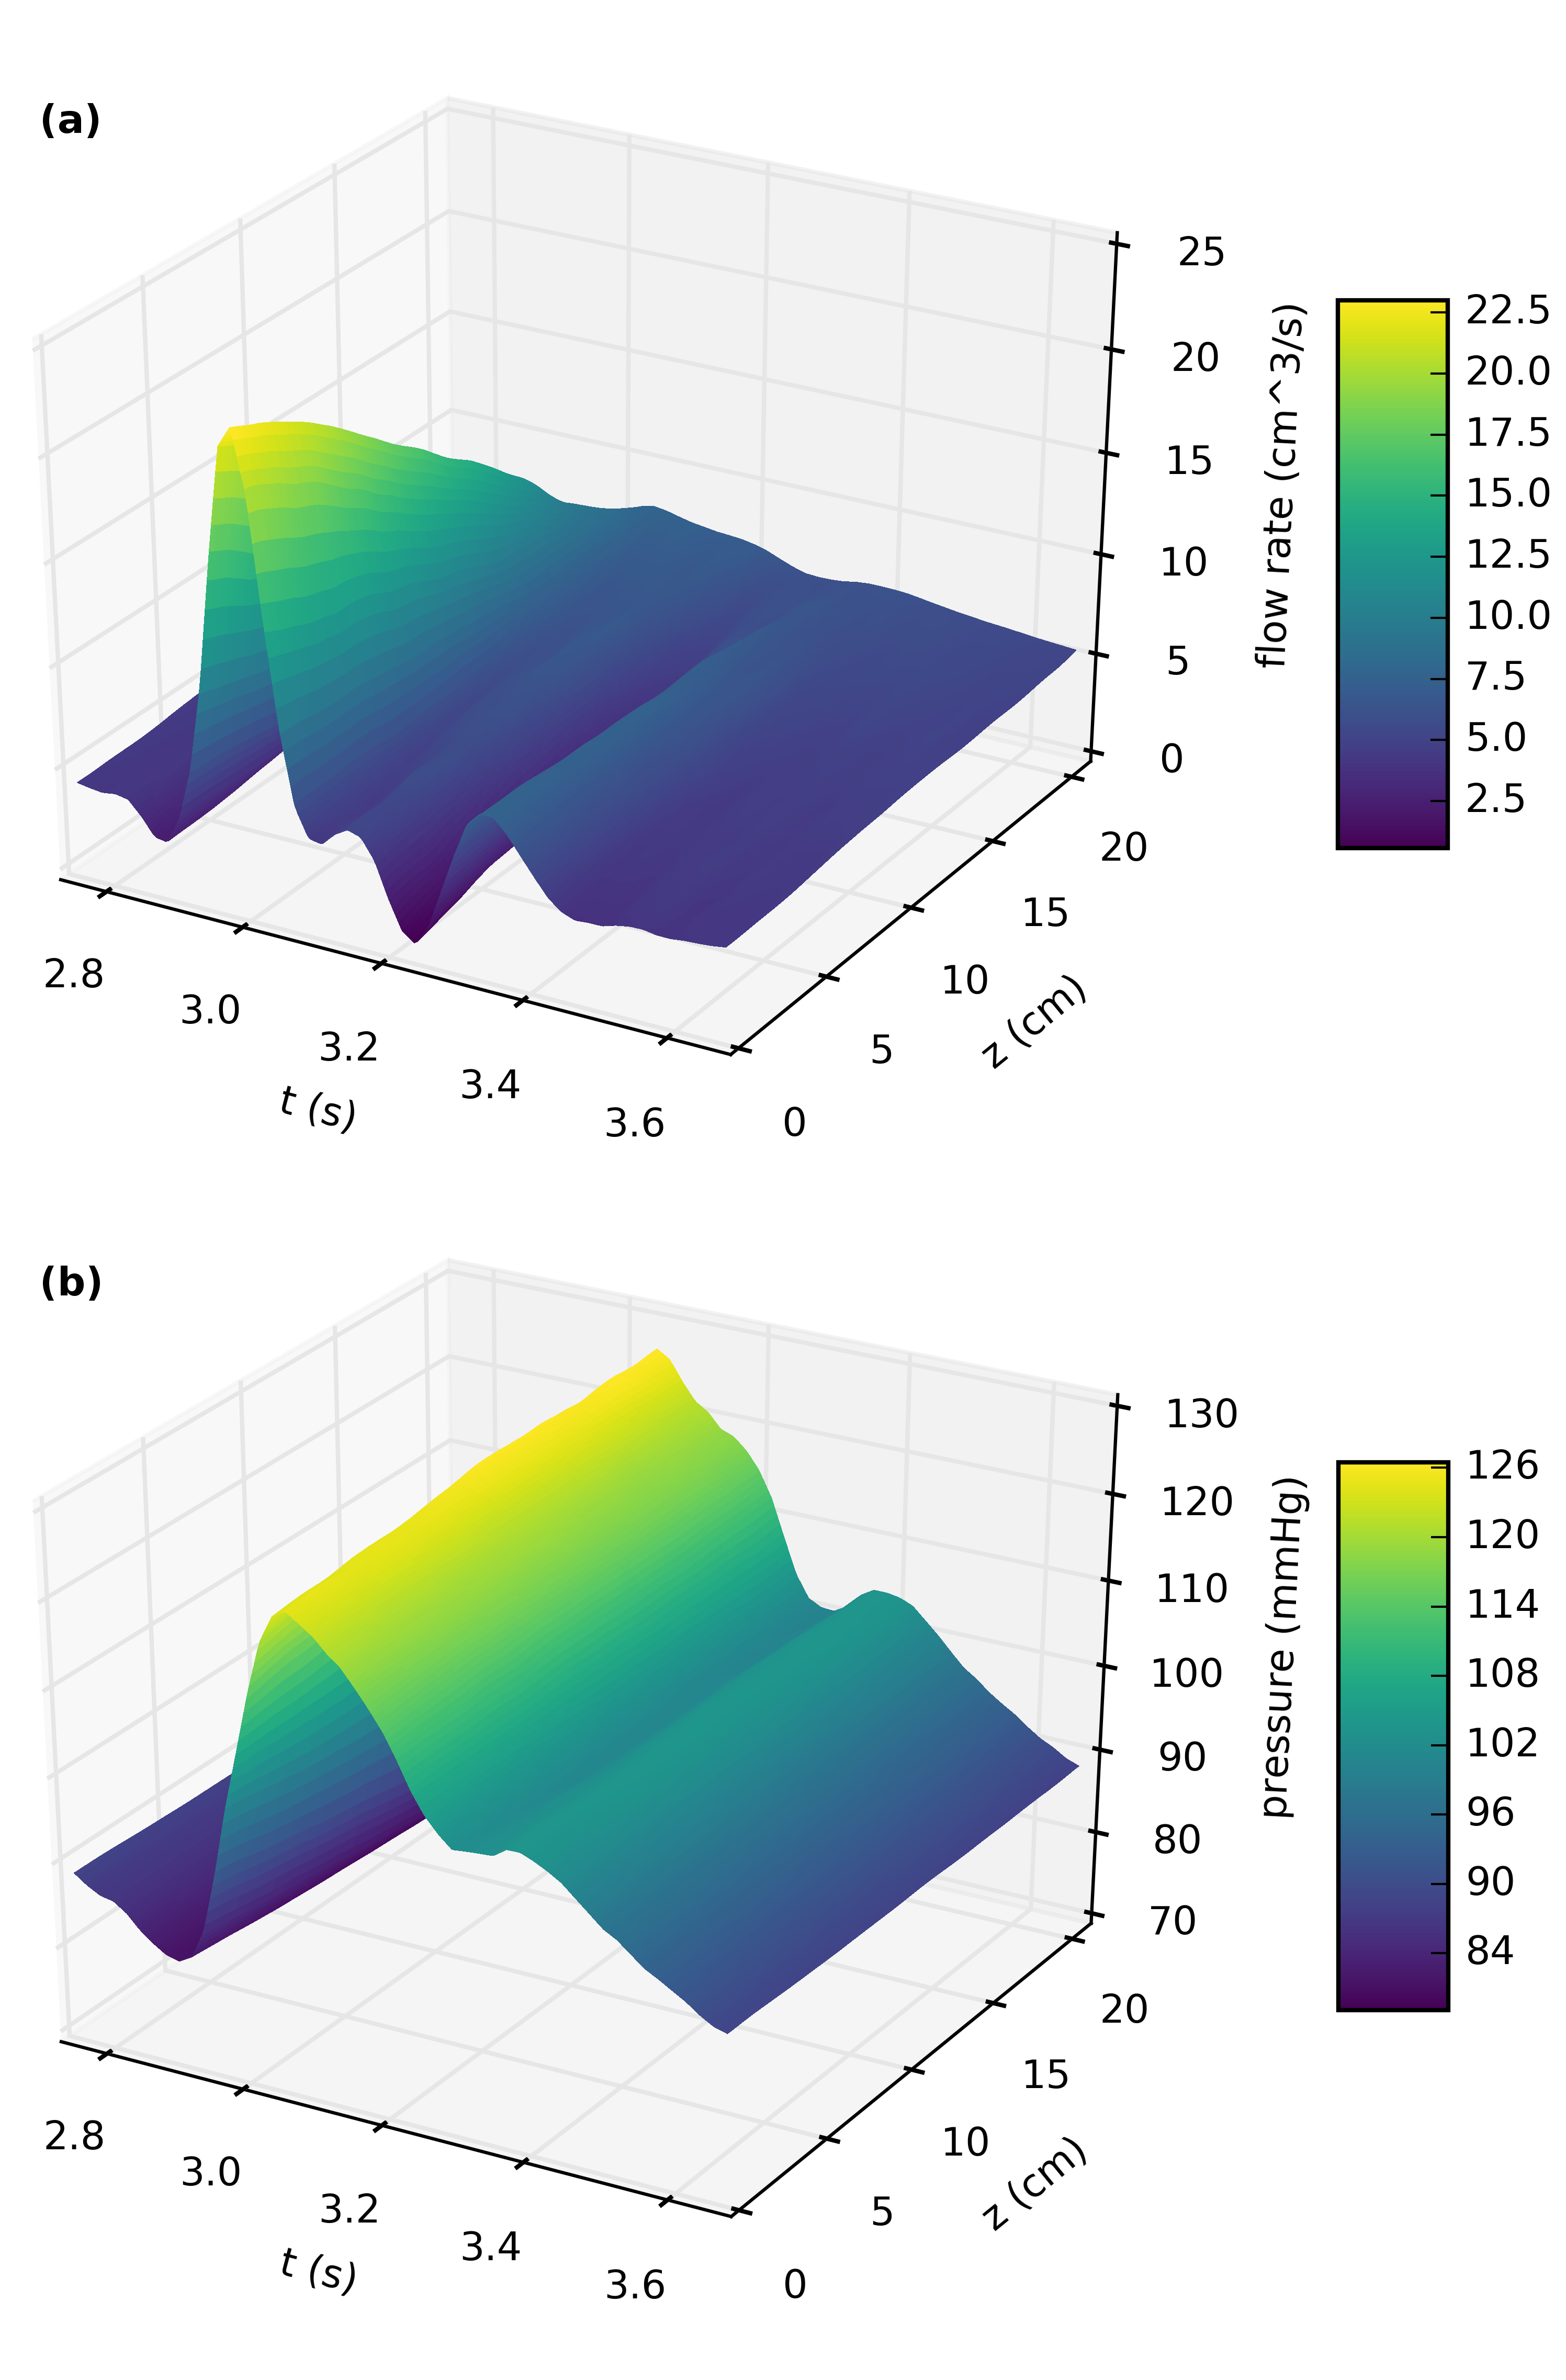
\includegraphics[width=\linewidth]{figures/cca_p_q.png}
  \caption{One pulse in the common carotid artery using VaMpy: a) flow rate, b) pressure. Comparison with the results for the same simulation in \cite{Kolachalama2007} validates the implementation of the blood flow equations in VaMpy.\label{fig:bifurcation}}
\end{figure}

The VaMpy Git repository contains unit tests to ensure functions perform as expected. Additionally, the file \texttt{bifurcation\_example.py} demonstrates VaMpy's performance by validating its results against results in \cite{Kolachalama2007} on the common carotid artery bifurcation. Whilst unit tests demonstrate that the functionality of the software meets expecations, validation against experimental results and other researchers' results ensures that the software additionally generates sensible output data and that parameters have been chosen sensibly. Users implementing arteries using other parameters than the ones tested in the example files in VaMpy should therefore always cross-check their results against experimental or other simulation results using the same parameters to ensure that the choice of parameters is realistic.

The solution computed using VaMpy is shown in Figure~\ref{fig:bifurcation} and matches the corresponding figures in \cite{Kolachalama2007}. Thus this example demonstrates that VaMpy performs as expected.

To execute the example run
\begin{verbatim}
python bifurcation_example.py bifurcation.cfg
\end{verbatim}
To plot the data created from the example run
\begin{verbatim}
python plot_example.py bifurcation.cfg
\end{verbatim}

The first version of VaMpy focusses on the simulation of a single bifurcation, i.~e. one parent vessel with two daughter vessels. The development of the first version of VaMpy was based on the simulation of flow through the middle cerebral artery in order to evaluate lymphatic drainage through the wall of the artery \cite{Diem2016a}, and for this purpose a single bifurcation was regarded sufficient. Validation on larger networks of arteries with multiple levels of bifurcations has therefore not been carried out yet, but is planned for the next release cycle. Additionally, it is planned to offer a choice of alternative outlet boundary conditions, such as the structured tree \cite{Olufsen2000,Cousins2014}. It has been demonstrated that by taking into account bifurcation pressure drops, the accuracy of reduced order models such as the system of equations \eqref{eq:conservation} can improve significantly compared to higher order models \cite{Chnafa2016}. This means that a similar accuracy of blood flow solutions could be achieved for 1D models compared to 2D or 3D models by increasing the depth of the arterial tree to be modelled.

\section*{(2) Availability}
\vspace{0.5cm}
\section*{Operating system}

VaMpy is compatible with any operating system that is compatible with Python 2.7 and the dependent packages.

\section*{Programming language}

VaMpy was written in and for Python 2.7 and above.

\section*{Additional system requirements}

There are no additional system requirements. However, the requirements for memory and processing power are dependent on the number of the grid points.

\section*{Dependencies}

NumPy, SciPy, Matplotlib, ConfigParser.

\section*{Software location:}


{\bf Archive}

\begin{description}[noitemsep,topsep=0pt]
	\item[Name:] GitHub
	\item[Persistent identifier:] https://github.com/akdiem/vampy/releases/tag/v1.0
	\item[Licence:] Three-Clause BSD
	\item[Publisher:]  Alexandra K. Diem
	\item[Version published:] v1.0
	\item[Date published:] 22/03/2017
\end{description}

{\bf Code repository}

\begin{description}[noitemsep,topsep=0pt]
	\item[Name:] GitHub
	\item[Persistent identifier:] https://github.com/akdiem/vampy
	\item[Licence:] Three-Clause BSD
	\item[Date published:] 26/04/2016
\end{description}

\section*{Language}

Python 2.7

\section*{(3) Reuse potential}

Modelling blood flow dynamics is a useful tool in vascular diseases research and 1D models provide good approximations. The method implemented in VaMpy is used by a variety of research groups \cite{Olufsen2000,Kolachalama2007,Itu2011} and therefore it is expected that the reuse potential for VaMpy is high, especially in multiscale simulations. Because the commonly accepted CSV file format is used for input and output data for VaMpy integration of results from VaMpy simulations with other third-party software packages is expected to be straightforward. For example, VaMpy could be used as a boundary condition for 3D simulations or constitute a part of multi-scale simulations.

The publication of this software additionally provides opportunities for other researchers to add functionality and because VaMpy has been validated on results published in the literature it simplifies and promotes reproducibility of results. The following features are planned for the next releases:

\begin{itemize}
\item asymmetric daughter vessel geometries with separate Windkessel parameters,
\item validation of the method on bifurcation networks larger than two levels and
\item integration of models of the dynamics of the artery wall.
\end{itemize}

The current release of VaMpy was developed to implement a bifurcation at the middle cerebral artery as part of a multi-scale model of lymphatic flow through the basement membrane embedded in the artery wall, which is relevant for resolving the mechanisms behind the onset and progression of Alzheimer's disease \cite{Diem2016a,Bakker2016}.

\section*{Acknowledgements}

The authors thank Maximilian Albert for advice and guidance on the use of GitHub repositories and Python code repository conventions.

\section*{Funding statement}

The development of this software was supported by an EPSRC Doctoral Training Centre grant (EP/G03690X/1).

\section*{Competing interests}

The authors declare that they have no competing interests.

\printbibliography

\vspace{2cm}

\rule{\textwidth}{1pt}

{ \bf Copyright Notice} \\
Authors who publish with this journal agree to the following terms: \\

Authors retain copyright and grant the journal right of first publication with the work simultaneously licensed under a  \href{http://creativecommons.org/licenses/by/3.0/}{Creative Commons Attribution License} that allows others to share the work with an acknowledgement of the work's authorship and initial publication in this journal. \\

Authors are able to enter into separate, additional contractual arrangements for the non-exclusive distribution of the journal's published version of the work (e.g., post it to an institutional repository or publish it in a book), with an acknowledgement of its initial publication in this journal. \\

By submitting this paper you agree to the terms of this Copyright Notice, which will apply to this submission if and when it is published by this journal.


\end{document}
